% !TeX program = lualatex
% !TeX encoding = utf8
% !TeX spellcheck = uk_UA
% !BIB program = biber

\documentclass[]{QChemPresent}
\usetikzlibrary{calligraphy}

\date{}
\let\vphi\varphi
\def\vxi{\vec{\xi}}
\begin{document}
%==============================================================================================

\begin{frame}[fragile]

		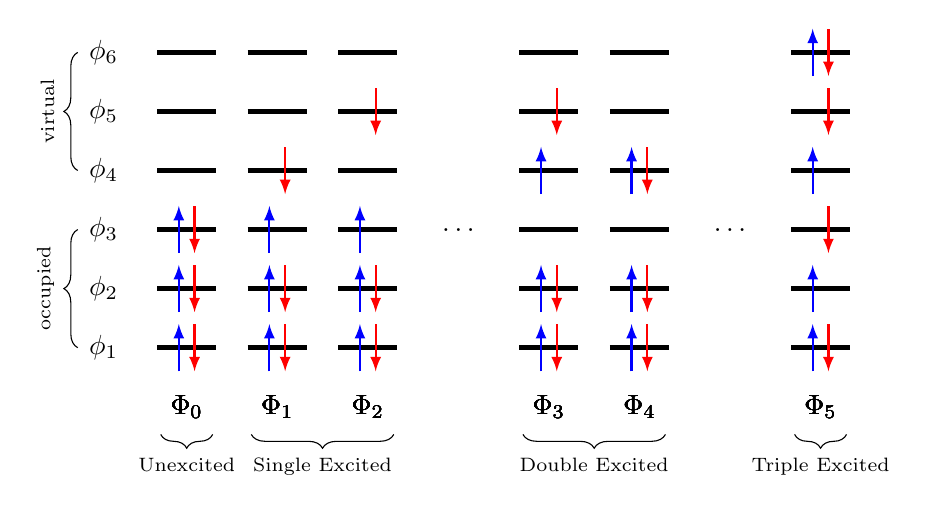
\begin{tikzpicture}[
				upspinarrow/.pic = {\draw[-latex, blue, thick] (0,-0.3) -- (0, 0.3);},
				downspinarrow/.pic = {\draw[latex-,red, thick] (0,-0.3) -- (0, 0.3);},
                updown/.style={insert path={
                    pic at ([xshift=-0.1cm]#1) {upspinarrow}
                    pic at ([xshift=+0.1cm]#1) {downspinarrow}
                }},
                 up/.style={insert path={
                    pic at ([xshift=-0.1cm]#1) {upspinarrow}
                }},
                 down/.style={insert path={
                    pic at ([xshift=+0.1cm]#1) {downspinarrow}
                }},
                curlybrace/.style = {decorate,decoration={brace,amplitude=5pt, mirror, raise=10pt}},
                curlybracel/.style = {decorate,decoration={brace,amplitude=5pt}},
			]

			\def\xshiftnode{1.15}
			\def\distance{0.75}
            \def\lofl{0.75}
            \foreach \i[count = \c from 0] in {1,...,3,5,6,8}{
                \foreach \j in {1,...,6}{
        			\draw[ultra thick]  (\i*\xshiftnode,\j*\distance)
                \ifnum\i=1 node[left=10pt] (phi\j) {$\phi_{\j}$}\fi -- coordinate (O\i\j) ++(\lofl,0);
                \node (Ph\c) at ({\i*\xshiftnode+0.5*\lofl}, 0) {$\Phi_{\c}$};
                }
            }
            \path[dotted] (O33.east) -- node {$\ldots$} (O53.west);
            \path[dotted] (O63.east) -- node {$\ldots$} (O83.west);
            \path [
                    updown=O11, updown=O12, updown=O13,
                    updown=O21, updown=O22, up    =O23, down=O24,
                    updown=O31, updown=O32, up    =O33, down=O35,
                    updown=O51, updown=O52, up    =O54, down=O55,
                    updown=O61, updown=O62, up    =O64, down=O64,
                    updown=O81, up    =O82, down  =O83, up  =O84, down=O85, updown=O86,
                  ];
                \draw [curlybrace]   (Ph0.west) -- (Ph0.east) node[midway, below=15pt, font=\scriptsize]{Unexcited};
                \draw [curlybrace]   (Ph1.west) -- (Ph2.east) node[midway, below=15pt, font=\scriptsize]{Single Excited};
                \draw [curlybrace]   (Ph3.west) -- (Ph4.east) node[midway, below=15pt, font=\scriptsize]{Double Excited};
                \draw [curlybrace]   (Ph5.west) -- (Ph5.east) node[midway, below=15pt, font=\scriptsize]{Triple Excited};

                \draw [curlybracel]   (phi1.west) -- (phi3.west) node[midway, font=\scriptsize, sloped, above=5pt]{occupied};

                \draw [curlybracel]   (phi4.west) -- (phi6.west) node[midway, font=\scriptsize, sloped, above=5pt]{virtual};

\end{tikzpicture}

\end{frame}

%============================================================================
\begin{frame}[fragile]{}{}
\begin{center}
    \begin{tikzpicture}[
				upspinarrow/.pic = {\draw[-latex, blue, thick] (0,-0.3) -- (0, 0.3);},
				downspinarrow/.pic = {\draw[latex-,red, thick] (0,-0.3) -- (0, 0.3);},
                updown/.style={insert path={
                    pic at ([xshift=-0.1cm]#1) {upspinarrow}
                    pic at ([xshift=+0.1cm]#1) {downspinarrow}
                }},
                 up/.style={insert path={
                    pic at ([xshift=-0.1cm]#1) {upspinarrow}
                }},
                 down/.style={insert path={
                    pic at ([xshift=+0.1cm]#1) {downspinarrow}
                }},
                ]
            \coordinate (s) at (0,0);
            \coordinate (p) at (4,0);
            \orbital[pos = {(s)},  scale = 2, pcolor = red,]{s}
            \path [updown=s];
			\orbital[pos = {(p)},  scale = 2, pcolor = red,]{pz}
            \pic at ([xshift=1cm]p) {upspinarrow};
            \orbital[pos = {(p)},  scale = 2, pcolor = blue,]{py}
            \pic at ([yshift=1cm]p) {downspinarrow};
%            \orbital[pos = {(0,0)},  scale = 2, pcolor = red,]{px}
	\end{tikzpicture}
\end{center}
\end{frame}
%============================================================================

\end{document}

%            \ifnum\i<4
%            pic[pos=0.35] {upspinarrow}  pic[pos=0.65] {downspinarrow}
%            \fi